\chapter{Inflationary Cosmology}
\label{chap:cos}

\section{Introduction}
\label{sec:cos:intro}
I assume a working knowledge of Einstein's theory of general relativity. Review the key concepts mostly to establish notation. Excellent references can be found in~\cite{Wald},~\cite{Hobson} \&~\cite{Dodelson}.

\section{Einstein's gravity}
\label{sec:cos:einsteins_gravity}
\begin{quote}
  {\em Spacetime tells matter how to move;\\ matter tells spacetime how to curve.}\hfill
  --- \johnwheeler{}
\end{quote}

Einstein's theory of general relativity accounts for gravity by removing it as a fundamental ``force'' and replacing it as an effect of spacetime itself. Objects and fields still interact with one another on a spacetime background via the usual forces (electromagnetic, strong and weak nuclear forces). The spacetime itself can be thought of as being curved, and the effect of gravitation is due to objects moving on paths through a curved spacetime. Finally, the curvature is influenced by the matter content of the spacetime.

The formalism of Einstein's gravity can be effectively summarised using the Einstein-Hilbert action. An action $S$ is written as a general relativistic integral over a Lagrangian density $\mathcal{L}$:\footnote{This should not be confused with a likelihood, also denoted with $\lik$.}
\begin{equation}
  S = \int d^4 x \sqrt{|g|} \mathcal{L}.
  \label{eqn:cos:generic_lagrangian}
\end{equation}
where the factor of $\sqrt{g}$, $g=\left|\det\left( g_{\mu\nu} \right)\right|$ ensures a relativistic volume element for integration.
We typically decompose the Lagrangian $\mathcal{L}$ into a gravitational and matter part:
\begin{align}
  \mathcal{L} &= \mathcal{L}_G + \mathcal{L}_M
  \label{eqn:cos:decomp}\\
  \mathcal{L}_G &= \frac{1}{2} \m^2 R
  \label{eqn:cos:L_grav}
\end{align}
where $R$ is the Ricci scalar and $\mathcal{L}_M$ is the portion of the Lagrangian pertaining to the material content of spacetime. Requiring that the action~\eqref{eqn:cos:generic_lagrangian} is extremal ($\delta S = 0$) yields Einstein's equations:
\begin{equation}
  G_{\mu\nu} = \frac{1}{\m^2}T_{\mu\nu},
  \label{eqn:cos:einsteins_equations}
\end{equation}
where
\begin{equation}
  T_{\mu\nu} = \frac{-2}{\sqrt{\abs{g}}}\frac{\delta}{\delta g^{\mu\nu}}\left( \sqrt{\abs{g} \mathcal{L}_M} \right)
  \label{eqn:cos:SET_fundamantal}
\end{equation}
is the stress energy tensor, and
\begin{equation}
  G_{\mu\nu} = R_{\mu\nu} - \frac{1}{2}g_{\mu\nu} R,
  \label{eqn:cos:einstein_tensor}
\end{equation}
is the Einstein tensor. The symmetries of the Einstein tensor~\eqref{eqn:cos:einstein_tensor} mean that there are in fact only six independent equations in~\eqref{eqn:cos:einsteins_equations}. Further, the fact that $\nabla^\mu G_{\mu\nu}=0$ means that the stress energy tensor is conserved:
\begin{equation}
  \nabla_\mu T^{\mu}_{\nu} = 0
  \label{eqn:cos:SET_conservation}
\end{equation}
This conservation equation can provide a fast means for deriving alternative rearragements of the Einstein equations.

\section{The smooth, expanding universe}
\subsection{Metric}
\begin{table}
  \centering
\begin{tabular}{ll}
 \toprule
  Symbol & Definition \\
 \midrule
 \midrule
  $t$ & cosmic time \\
  $\chi$ & Comoving radial coordinate \\
  $\theta$ & polar angle \\
  $\phi$ & azimuthal angle \\
  $\Omega$ & solid angle \\
  $a$ & cosmic scale factor \\
  $k=+1$ & open universe \\
  $k=0$ & flat universe \\
  $k=-1$ & closed universe \\
 \bottomrule
\end{tabular}
\caption{Definitions of terms in the FRW metric}\label{tab:cos:metric}
\end{table}

On the largest scales, the universe is observed to be {\em homogeneous\/} and {\em isotropic}. This provides a good 0\textsuperscript{th}-order approximation to our actual universe. Making these assumptions, the metric can take one of three generic forms:
\begin{align}
  ds^2 &= dt^2 - a{(t)}^2\left( d\chi^2 + S_k^2{(\chi)} d\Omega \right)
  \label{eqn:cos:FRW_metric}\\
  d\Omega &= d\theta^2 + \sin^2\theta d\phi^2
  \label{eqn:cos:angle_element}\\
  S_k^2(\chi) &=
  \left\{
  \begin{array}{rl}
    \sin^2\chi &: k=+1 \\
    \chi^2 &: k=0 \\
    \sinh^2\chi &: k=-1. \\
  \end{array}
  \right.\label{eqn:cos:S_def}
\end{align}
The definitions of these terms can be found in Table~\ref{tab:cos:metric}. The scale factor $a(t)$ connects {\em comoving coordinates\/} $\chi$ with {\em physical coordinates}. Comoving variables can be thought of as a time-independent grid, which expand with the universe (Figure~\ref{fig:cos:comoving_vs_physical}). Physical coordinates are found by multiplying via the scale factor $a(t)$ to account for the effect of the expansion of the universe.
\begin{figure}
  \centering
  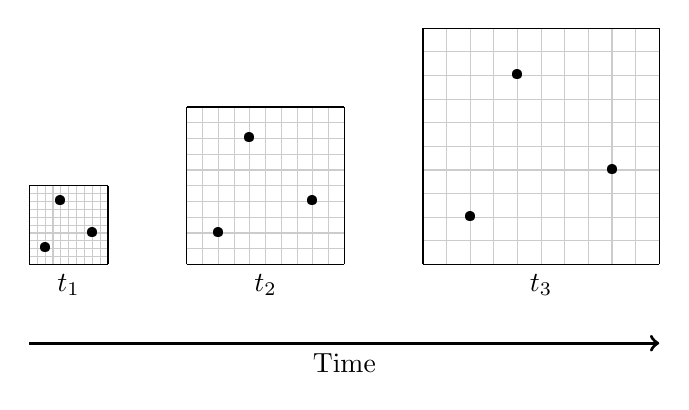
\begin{tikzpicture}
  % Draw the grids
  \draw[step=0.1,opacity=0.2] (0,0) grid (1,1);
  \draw[step=1] (0,0) grid (1,1);

  \draw[xshift=2cm,scale=2,step=0.1,opacity=0.2] (0,0) grid (1,1);
  \draw[xshift=2cm,scale=2,step=1] (0,0) grid (1,1);

  \draw[xshift=5cm,scale=3,step=0.1,opacity=0.2] (0,0) grid (1,1);
  \draw[xshift=5cm,scale=3,step=1] (0,0) grid (1,1);

  % Arrow of time
  \path[->, very thick] 
  (0,-1) 
  edge node[below] {Time}
  (8,-1);

  % Time Labels
  \node[below] at (0.5,0) {$t_1$};
  \node[below] at (3,0) {$t_2$};
  \node[below] at (6.5,0) {$t_3$};

  \def\xa{0.2} \def\ya{0.2}
  \def\xb{0.8} \def\yb{0.4}
  \def\xc{0.4} \def\yc{0.8}
  \def\object{\textbullet}

  \node[] (a1) at (\xa,\ya) {\object};
  \node[] (b1) at (\xb,\yb) {\object};
  \node[] (c1) at (\xc,\yc) {\object};

  \node[] (a2) at ({\xa*2 + 2},{\ya*2}) {\object};
  \node[] (b2) at ({\xb*2 + 2},{\yb*2}) {\object};
  \node[] (c2) at ({\xc*2 + 2},{\yc*2}) {\object};

  \node[] (a3) at ({\xa*3 + 5},{\ya*3}) {\object};
  \node[] (b3) at ({\xb*3 + 5},{\yb*3}) {\object};
  \node[] (c3) at ({\xc*3 + 5},{\yc*3}) {\object};


\end{tikzpicture}

  \caption{Comoving vs.\ physical coordinates.\label{fig:cos:comoving_vs_physical}}
\end{figure}




\subsection{Dynamics}
In order to obtain the equations governing $a(t)$ and thus the dynamics of the universe, we must make some assumptions about the universes contents. For a smooth universe, one may model its contents as a collection of non-interacting, comoving, uniform, perfect fluids. A perfect fluid in thermodynamic equilibrium has stress-energy tensor:
\begin{equation}
  T^{\mu\nu} = (P+\rho)u^{\mu}u^{\nu} - P g^{\mu\nu} + \Sigma^{\mu\nu}
  \label{eqn:cos:SET_perfect_fluid}
\end{equation}
where $\rho$ is the energy density, $P$ is the pressure, $u^\mu$ is the four velocity of the fluid, and $\Sigma^{\mu\nu}$ is a traceless, symmetric, anisotropic stress term. In accordance with the cosmological principle, we shall assume that in the comoving frame the fluid is stationary ($u^\mu = [1,\bzero]$), and uniform ($\rho=\rho(t),P=P(t)$), with no anisotropy $\Sigma=0$.  

Applying the metric~\eqref{eqn:cos:FRW_metric} to the Einstein equations~\eqref{eqn:cos:einsteins_equations}, with the stress-energy tensor~\eqref{eqn:cos:SET_perfect_fluid} one finds:
\begin{align}
  \dot{H}+H^2 &= 
  -\frac{1}{6\m^2}\left( \rho + 3P\right), 
  \label{eqn:cos:Raychaudhuri}
  \\
  H^2 &= 
  \frac{1}{3\m^2}\rho - \frac{k}{a^2}, 
  \label{eqn:cos:Friedmann}
\end{align}
%
where $H=\dot{a}/a$ is the Hubble parameter and a dot denotes differentiation with respect to cosmic time, $\dot{f}\equiv df/dt$. These are termed the {\em Raychaudhuri\/} and {\em Friedmann\/} equations respectively, and implicitly govern the dynamics of the scale factor $a(t)$. It should be noted that these equations are not complete, as additionally one requires an equation of state linking $\rho$ and $P$.

\subsection{Simple solutions}
A reasonable model for the universe we observe today is as a multi-component fluid, each with its own simple equation of state:
\begin{equation}
  \rho = \sum_i \rho_i, \qquad P = \sum_i P_i, \qquad P_i = w_i \rho_i
  \label{eqn:cos:multi_component}
\end{equation}
where $w_i$ is the equation of state parameter. In our universe, we observe matter $(w=0)$, radiation $(w=\frac{1}{3})$ and dark energy $(w=-1)$. We can also notationally model the curvature's scale-factor contribution of $-\frac{k}{a^2}$ as a cosmological fluid with $w=-\frac{1}{3}$. Applying these equations of states, equations~\eqref{eqn:cos:Raychaudhuri} and~\eqref{eqn:cos:Friedmann} may be re-cast as an equation purely in $a$:
\begin{equation}
  {\left( \frac{H}{H_0} \right)}^2 \equiv 
  \frac{1}{H_0^2}{\left( \frac{\dot{a}}{a} \right)}^2 =
  \Omega^\text{(rad)}_0 a^{-4} +
  \Omega^\text{(mat)}_0 a^{-3} + 
  \Omega^\text{(curv)}_0 a^{-2} +
  \Omega^\text{(de)}_0  
  \label{eqn:cos:expansion_history}
\end{equation}
where quantities subscripted with $0$ indicate the present day $(t=t_0)$ value of the parameter, the present scale factor is chosen to be unity $(a(t_0)=1)$, and the density parameter $\Omega$ is defined as:
\begin{equation}
  \Omega = \frac{\rho}{3\m^2H^2},
\end{equation}
which measures the fraction of of the critical density $\rho_c = 3\m^2H^2$ taken up by a given component. This equation cannot be analytically solved in this form, but if one assumes that one component is dominant, and the rest negligible, then one recovers the solution:
\begin{equation}
  a  \propto
  \left\{
  \begin{array}{ll}
    t^{2/3(w+1)} &: w\ne-1\\
    e^{H_0 t} &: w=-1.\\
  \end{array}
  \right.
\end{equation}
We can see immediately that in a universe dominated by dark energy $(w=-1)$ the expansion is exponential, and in one dominated by radiation $(w=1/3)$, that $a\propto t^{1/2}$, which is a slower expansion than one dominated by matter $a\propto t^{1/3}$. In our universe, where we observe that it is approximately flat, $\Omega_0^{\text{(curv)}}\approx0$, matter now vastly outweighs radiation, and is of the same order of magnitude as dark energy, ${\Omega_0^{\text{(de)}} \approx \Omega_0^{\text{(mat)}} \gg \Omega_0^{\text{(rad)}}}$, we expect an expansion history of the form shown in Figure~\ref{fig:cos:expansion_history}.

\begin{figure}
  \centering
  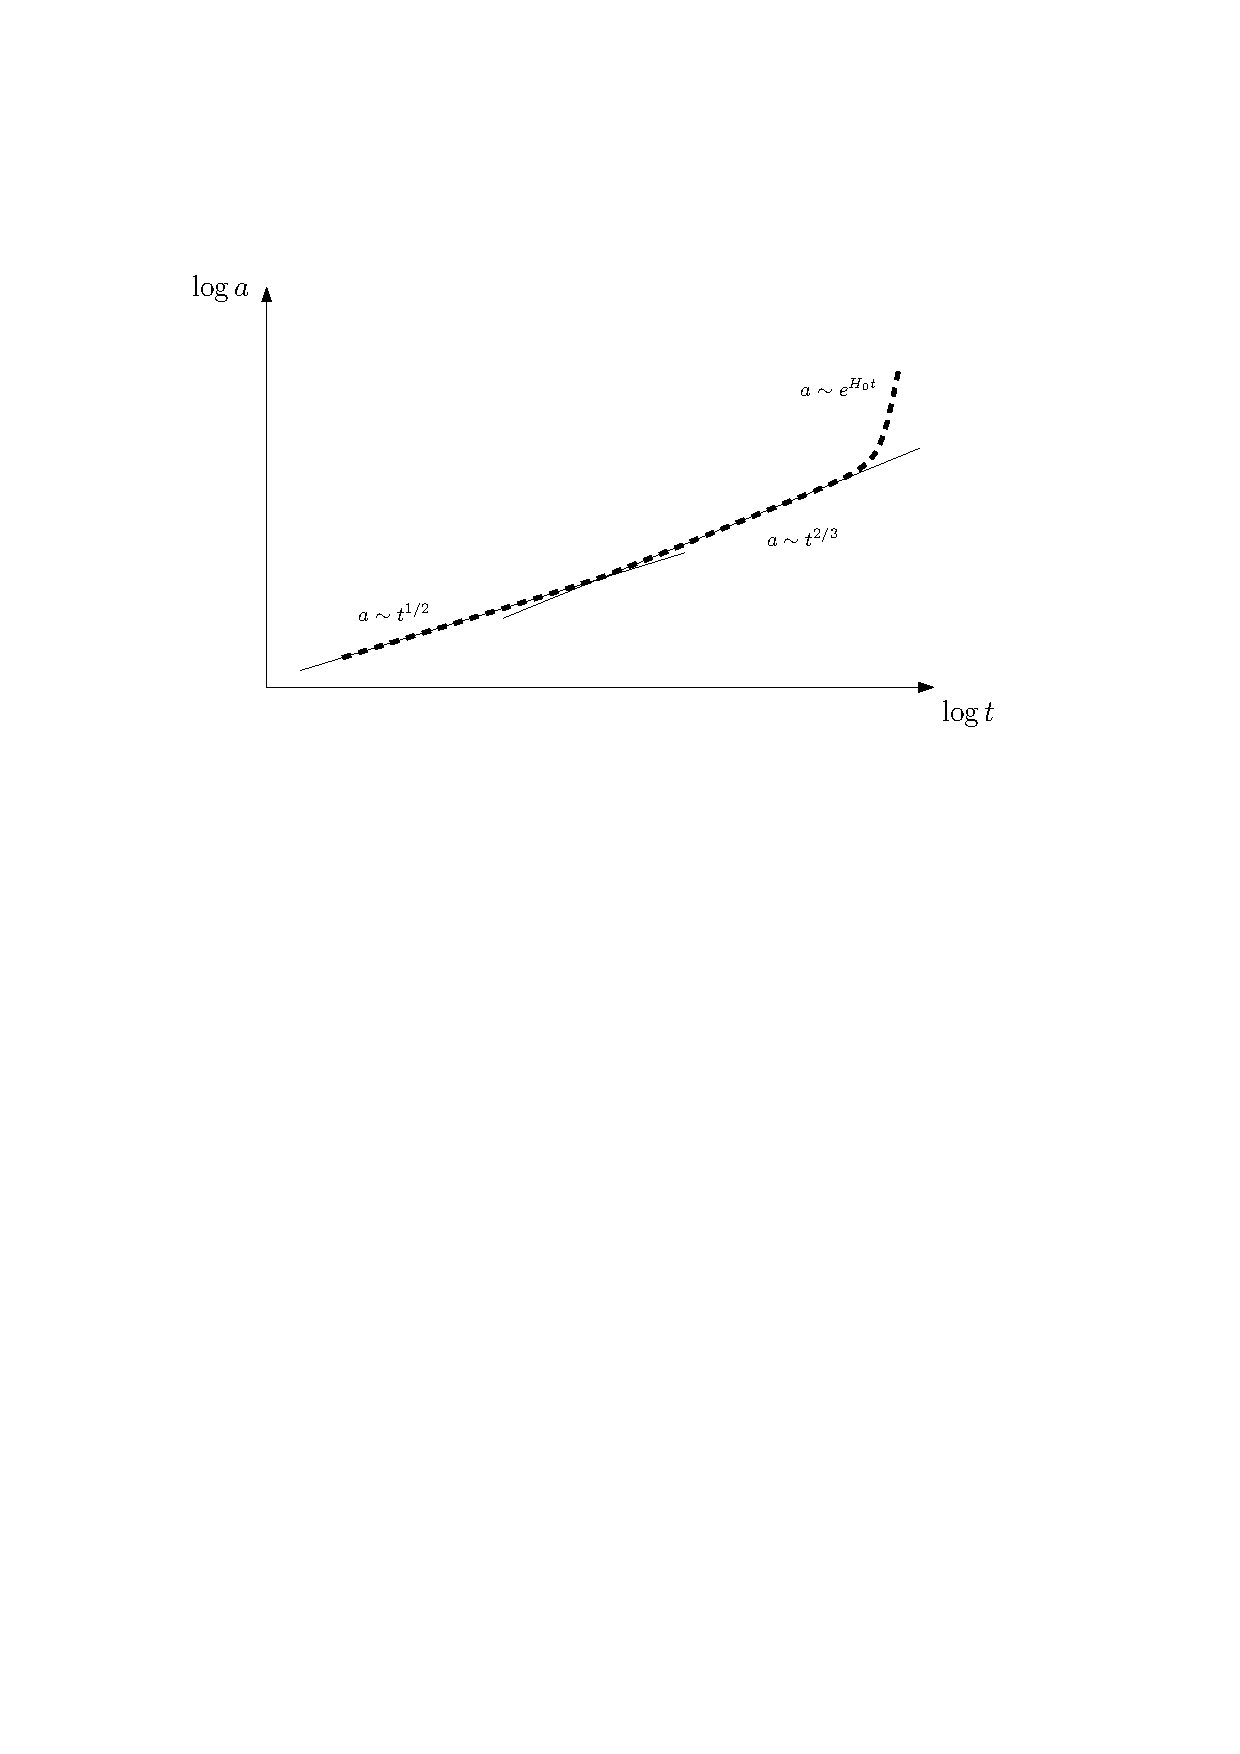
\includegraphics[width=\textwidth]{expansion_history}
  \caption{The approximate expansion history of our universe.\label{fig:cos:expansion_history}}
\end{figure}


\section{Conformal time and redshift}
\subsection{Conformal time $\eta$}

It convenient to define conformal time as:
\begin{equation}
  \eta = \int \frac{dt}{a},
  \label{eqn:cos:conformal_time}
\end{equation}
so that the line element becomes:
\begin{equation}          
  ds^2 = a(\eta)\left( d\eta^2 - dX^2 \right).
  \label{eqn:cos:flat_FRW}
\end{equation}
where $dX^2 = d\chi^2 + S_k^2(\chi) d\Omega$.
This is often analytically useful, but physically conformal time corresponds to a time coordinate in which photons appear as if they were in flt space: If we consider (without loss of generality) radially travelling photons $d\Omega=0$ the line element is simply:
\begin{equation}          
  ds^2 = a(\eta)\left( d\eta^2 - d\chi^2 \right).
  \label{eqn:cos:flat_FRW}
\end{equation}
and the metric is conformally equivalent to two-dimensional Minkowski space\footnote{Hence the name ``conformal time''.}. We have thus removed all of the complexities of curvature and comoving coordinates. Since photons have a null trajectory, $ds^2=0\Rightarrow d\eta = \pm d\chi$, and therefore  travel in straight lines on spacetime diagrams with $\eta$ and $\chi$ as axes. This considerably simplifies most pictures.
Alternatively, conformal time is the time measured by a small light clock that expands comovingly with the universe. It can therefore be thought of as a ``comoving'' time, in analogy with comoving spatial coordinates.

\subsection{Redshift $z$}
We now show that the expansion of the universe causes the wavelengths of a photons to increase: Photons have a four-momentum proportional to their wavevector $p^\mu \propto k^\mu$. Since the FRW metric has no explicit $\chi$-dependence for radially travelling photons, $p_\chi$ is conserved: $p_\chi(t_1) = p_\chi(t_2)$. Using the metric to raise the indices, one finds that $p^\chi(t_2)/a(t_2)=p^\chi(t_1)/a(t_1)$. Identifying ${p^\chi \propto k^r \propto \lambda^{-1}}$ where $\lambda$ is the wavelength of the photon, one finds:
\begin{equation}
  \frac{\lambda_2}{\lambda_1} = \frac{a_2}{a_1},
\end{equation}
and thus the wavelengths of photons increase with the expansion of the universe. Physically, the stretching of spacetime stretches the wavelengths of photons.
The redshift $z$ of the photon from some early time $t_1$, relative to the current epoch $t_0$, is defined as usual as:
\begin{equation}
  z = \frac{\lambda_0-\lambda_1}{\lambda_1},
\end{equation}
which gives a relation between the redshift of a photon and the scale factor:
\begin{equation}
  a = \frac{1}{1+z}.
\end{equation}
Since redshift is a physically observable quantity, it provides a cosmology-independent measure of the epoch of the universe (Table~\ref{tab:cos:universe_timeline}).
\begin{table}
  \centering
\begin{tabular}{ll}
 \toprule
  Epoch & Redshift \\
 \midrule
 \midrule
 Matter-radiation equality &
 $z\sim3400$
 \\
 Recombination &
 $z\sim1089$
 \\
 Dark ages &
 $20<z<1089$
 \\
 First stars &
 $z\sim20$
 \\
 Reionisation &
 $6<z<20$
 \\
 Dark energy-matter equality &
 $z=0.4$
 \\
 Now &
 $z=0$
 \\
 \bottomrule
\end{tabular}
\caption{Recent history of the universe. As redshifts are observable quantities, they should not depend on the specific contents of the universe, and provide a robust measure of cosmic epoch.}\label{tab:cos:universe_timeline}
\end{table}

\section{The cosmic microwave background}
As we turn telescopes on objects further away from earth, we begin to look appreciably back in time. The radiation from these objects has taken so long to reach us that we can observe the universe in a much younger state than it is now. The furthest galaxies imaged by the Hubble space telescope are more than 13 billion years old. Many of these objects are so far away that they have redshifted out of the visible spectrum and into the infra-red. If we look beyond these stars, we enter the dark ages, before the first stars had turned on. This would appear to be the end of the observational story.

However, from behind the dark ages, there is a background of microwaves. These would originally have been emitted as X-rays, but have redshifted all the way down to the microwave end of the spectrum.\footnote{Incidentally, this means that at around redshift $3<z<7$, the universe would have been bathed in optical light. However, it would have been at too low an intensity to be visible to the naked eye. Assuming a threshold of the human eye of $10^{-6}\mathrm{cd}\;\mathrm{m}^{-2}$, the CMB would stop being visible at $z\sim200$, at which point it would have been white.}. This uniform backdrop of radiation is our direct image of the universe as it was at redshift $z\sim1000$, when the universe was a mere $300,000$ years old.

Since its first (accidental) detection in 1964 by~\cite{PenziasWilson}, a succession of hundreds of microwave telescopes, both on the ground and in space, have sharpened our image of this (Figure~\ref{fig:cos:satellites}).
\begin{figure}
  \centering
  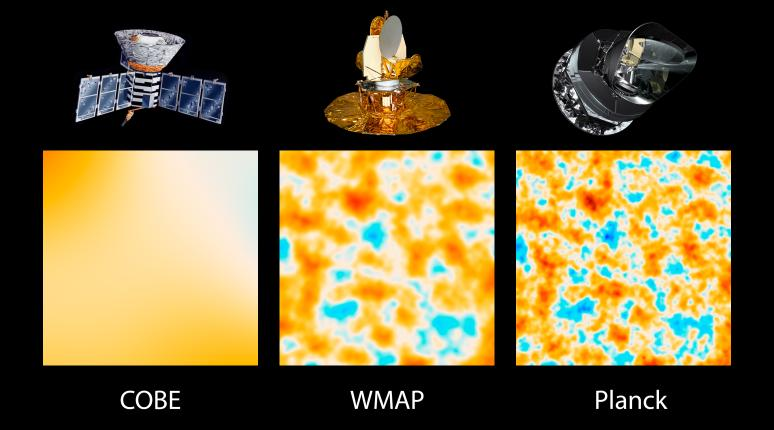
\includegraphics[width=\textwidth]{satellites}
  \caption{Microwave satellite pictures.\protect\footnote{Image credit:NASA/JPL-Caltech/ESA}}\label{fig:cos:satellites}
\end{figure}
The cosmic microwave background (CMB) is found to be:
\begin{enumerate}
  \item Isotropic to one part in $10^{5}$.
  \item A near perfect blackbody spectrum, with $T_0=2.7254(5)$.
  \item Anisotropic with non-trivial power spectrum.
\end{enumerate}

\section{The horizon and flatness problems}
The near-perfect isotropy of the CMB presents a problem. In 

One may think of this in terms of initial conditions\footnote{Specifically Cauchy initial conditions}, by stating that on some early spatial slice of the universe, the value of $X$ and $\dot{X}$ was extremely uniform, corresponding to the horizon and flatness problems respectively. 

\begin{equation}
  \eta = \int \frac{dt}{a} = \int \frac{da}{a^2H}
\end{equation}
Modelling as a single component universe with equation of state parameter $w$, equation~\eqref{eqn:cos:expansion_history} yields:
\begin{equation}
  H = H_0a^{-3(1+w)/2} \Rightarrow \eta =\frac{a^{(1+3w)/2}}{H_0(1+3w)/2}%\propto a^{(1+3w)/2} %
\end{equation}
For conventional matter $(w\ge0)$, this means that $\eta$ increases with time. Now, for photons:
\begin{equation}
  \Delta\chi = \chi_2 - \chi_1 = \eta_2 - \eta_1 = \Delta\eta
\end{equation}
represents the particle horizon, i.e. the furthest apart\ldots 

\begin{figure}
  \centering
  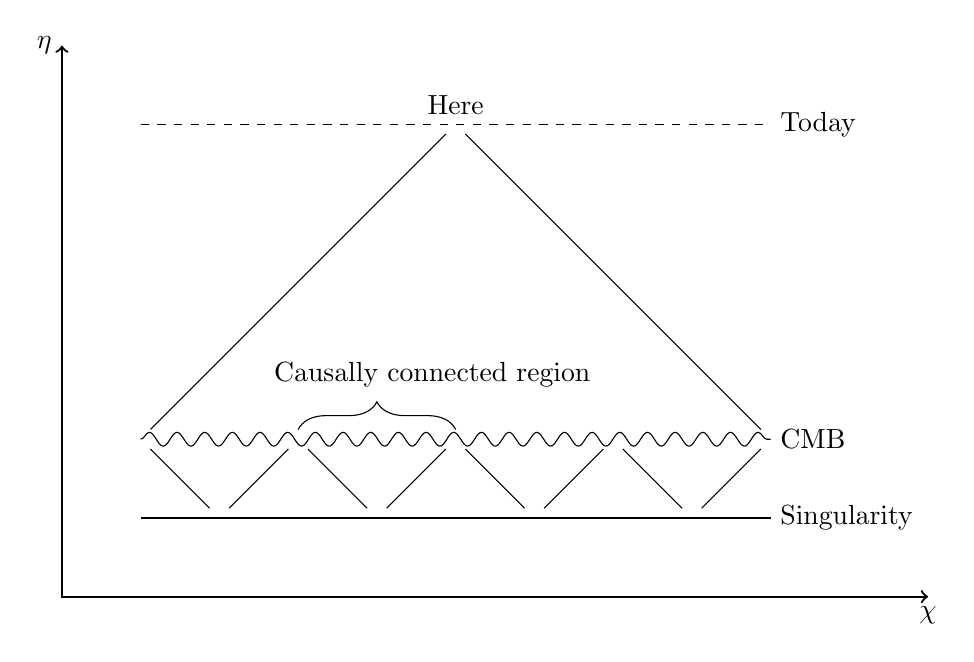
\begin{tikzpicture}
  \draw [<->,thick] (0,7) node (yaxis) [left] {\(\eta\)}
  |- (11,0) node (xaxis) [below] {\(\chi\)};

  % CMB

  % singularity
  \draw[] (1,1) -- (9,1) node [right] {Singularity};
  \draw[decorate,decoration=snake] (1,2) node (CMBl) {}  -- (9,2) node (CMBr) [right] {CMB};
  \draw[dashed] (1,6) -- (9,6) node [right] {Today};

  % causal contacts
  \draw (2,1) node (s1) {};
  \draw (4,1) node (s2) {};
  \draw (6,1) node (s3) {};
  \draw (8,1) node (s4) {};

  \draw (1,2) node (c1) {};
  \draw (3,2) node (c2) {};
  \draw (5,2) node (c3) {};
  \draw (7,2) node (c4) {};
  \draw (9,2) node (c5) {};
  \draw (5,6) node (now) {};

  
  \draw (c1) -- (s1) -- (c2);
  \draw (c2) -- (s2) -- (c3);
  \draw (c3) -- (s3) -- (c4);
  \draw (c4) -- (s4) -- (c5);

  \draw (c1) -- (now) -- (c5);
  \draw (now) node [above] {Here};

  \draw [decorate,decoration={brace,amplitude=10pt}]
  (c2.north) -- (c3.north) node [black,midway,yshift=20pt,xshift=20pt] {Causally connected region};

\end{tikzpicture}

  \caption{The horizon problem. From our position, we observe the CMB as a surface at some earlier time. The homogeneity of the CMB suggests that there must have been some physical mechanism to smooth it out. However, in cosmologies with traditional matter, there is not enough time before the CMB to allow this to occur. In fact, the CMB appears to be made up of causally disconnected regions. There is thus no dynamical reason as to why these disconeccetd regions should show such similar physical conditions. As a rough guideline, a causal patch is roughly a thumb-width on the sky.}\label{fig:cos:horizon_problem}
\end{figure}

\begin{figure}
  \centering
  \begin{tikzpicture}
  \draw [<->,thick] (0,7) node (yaxis) [left] {\(\eta\)}
  |- (11,-3) node (xaxis) [below] {\(\chi\)};

  % CMB

  % singularity
  %\draw[] (1,-4) -- (9,-4) node [right] {Singularity};
  \draw[decorate,decoration=snake] (1,2) node (CMBl) {}  -- (9,2) node (CMBr) [right] {CMB};
  \draw[dashed] (1,6) -- (9,6) node [right] {Today};

  % causal contacts
  \draw (2,1) node (s1) {};
  \draw (8,1) node (s4) {};

  \draw (1,2) node (c1) {};
  \draw (9,2) node (c5) {};
  \draw (5,6) node (now) {};
  \draw (5,-2) node (then) {};

  
  \draw (c1) -- (now) -- (c5);
  \draw (c1) -- (then) -- (c5);
  \draw (now) node [above] {Here};
  \draw (now) node [above] {Here};

\end{tikzpicture}

  \caption{Horizon problem resolved.\label{fig:cos:horizon_problem_resolved}}
\end{figure}

\section{An accelerating universe}
\section{Inflation}
The canonical way to explain this early accelerated phase is via the phenomenon of {\em inflation}. This early accelerated phase will have occurred when the universe was at extremely high energy, which suggests that we should turn to particle physics phenomenology.
It turns out if we consider even the most simple particle physics models, these are capable of generating a sustained accelerated phase in the context of general relativity.

\subsection{Basic theory}
Consider the Lagrangian:
\begin{equation}
  \mathcal{L}_\phi = \frac{1}{2}\nabla^\mu\phi\nabla_\mu\phi - V(\phi) 
  \label{eqn:cos:scalar_field_lagrangian}
\end{equation}
This represents a scalar field $\phi$, minimally coupled to gravity with some unspecified potential $V$.  Inserting this into~\eqref{eqn:cos:SET_fundamantal} yields a stress energy tensor of:
\begin{equation}
  T^{\mu}_{\nu} = \nabla^\mu\phi\nabla_\nu\phi - \left( \frac{1}{2}\nabla^\alpha\phi \nabla_\alpha\phi - V(\phi)  \right)\delta^{\mu}_{\nu}
  \label{eqn:cos:scalar_field_SET}
\end{equation}
If we initially assume in accordance with the cosmological principle that the field has no spatial dependence $\phi = \phi(t)$, then the stress energy tensor becomes:
\begin{align}
  T^{0}_{0} &=\frac{1}{2}\dot\phi^2 + V(\phi) = \rho 
  \label{eqn:cos:scalar_field_rho}\\
  T^{i}_{j} &=-\left[ \frac{1}{2}\dot\phi^2 - V(\phi)\right]\delta^{i}_{j} = -P\delta^{i}_{j}
  \label{eqn:cos:scalar_field_P}
\end{align}
Thus, a scalar field acts as a perfect fluid with pressure and density as shown above. In order to derive the equation of state, we need to generate an equation of motion for $\phi$. This can be done other by extremising $S_\phi = \int d^4 x \sqrt{|g|} \mathcal{L}_\phi$, or by applying the continuity equation~\eqref{eqn:cos:SET_conservation} to the stress energy tensor~\eqref{eqn:cos:scalar_field_SET}: 
\begin{equation}
  0 = \ddot{\phi} + 3 H \dot{\phi} + \frac{d}{d\phi}V(\phi)
  \label{eqn:cos:KG}
\end{equation}
The middle term involving $H$ is the term that arises as a result of including the effects of gravity (i.e.\ an expanding universe). The homogenous value of the scalar field $\phi$ satisfies the equation of a harmonic oscillator in potential $V(\phi)$ with a frictional term $H$.
To get an equation for $H$, we use the Raychaudhuri equation~\eqref{eqn:cos:Raychaudhuri} along with our formulae~\eqref{eqn:cos:scalar_field_rho}~\&~\eqref{eqn:cos:scalar_field_P} for $\rho$ and $P$, to find
\begin{equation}
  \dot{H}+H^2 = -\frac{1}{3\m^2}\left(\dot{\phi}^2-V(\phi)\right)
  \label{eqn:cos:ray_scalar}
\end{equation}
Equation~\eqref{eqn:cos:KG} represents space telling matter how to move and equation~\eqref{eqn:cos:ray_scalar} represents matter telling space how to curve respectively. These are tightly coupled, and result in far less trivial behaviour compared with a simple perfect fluid.


\subsection{Phenomenology}
One way to trigger an accelerated phase is to set the inflaton as trapped in a false vacuum (Figure~\ref{fig:cos:potential}). This sets $\dot{\phi}=0$, $V(\phi)=V_0$ and therefore $H=H_0=V_0/3\m^2$ and $a\sim e^{H_0t}$, which is an exponential and therefore accelerated expansion. However, to end this accelerated phase, the inflaton would have to tunnel quantum mechanically out of its false vacuum. It turns out that the false vacuum is too stable, and results in unphysical predictions.

\begin{figure}
  \centering
  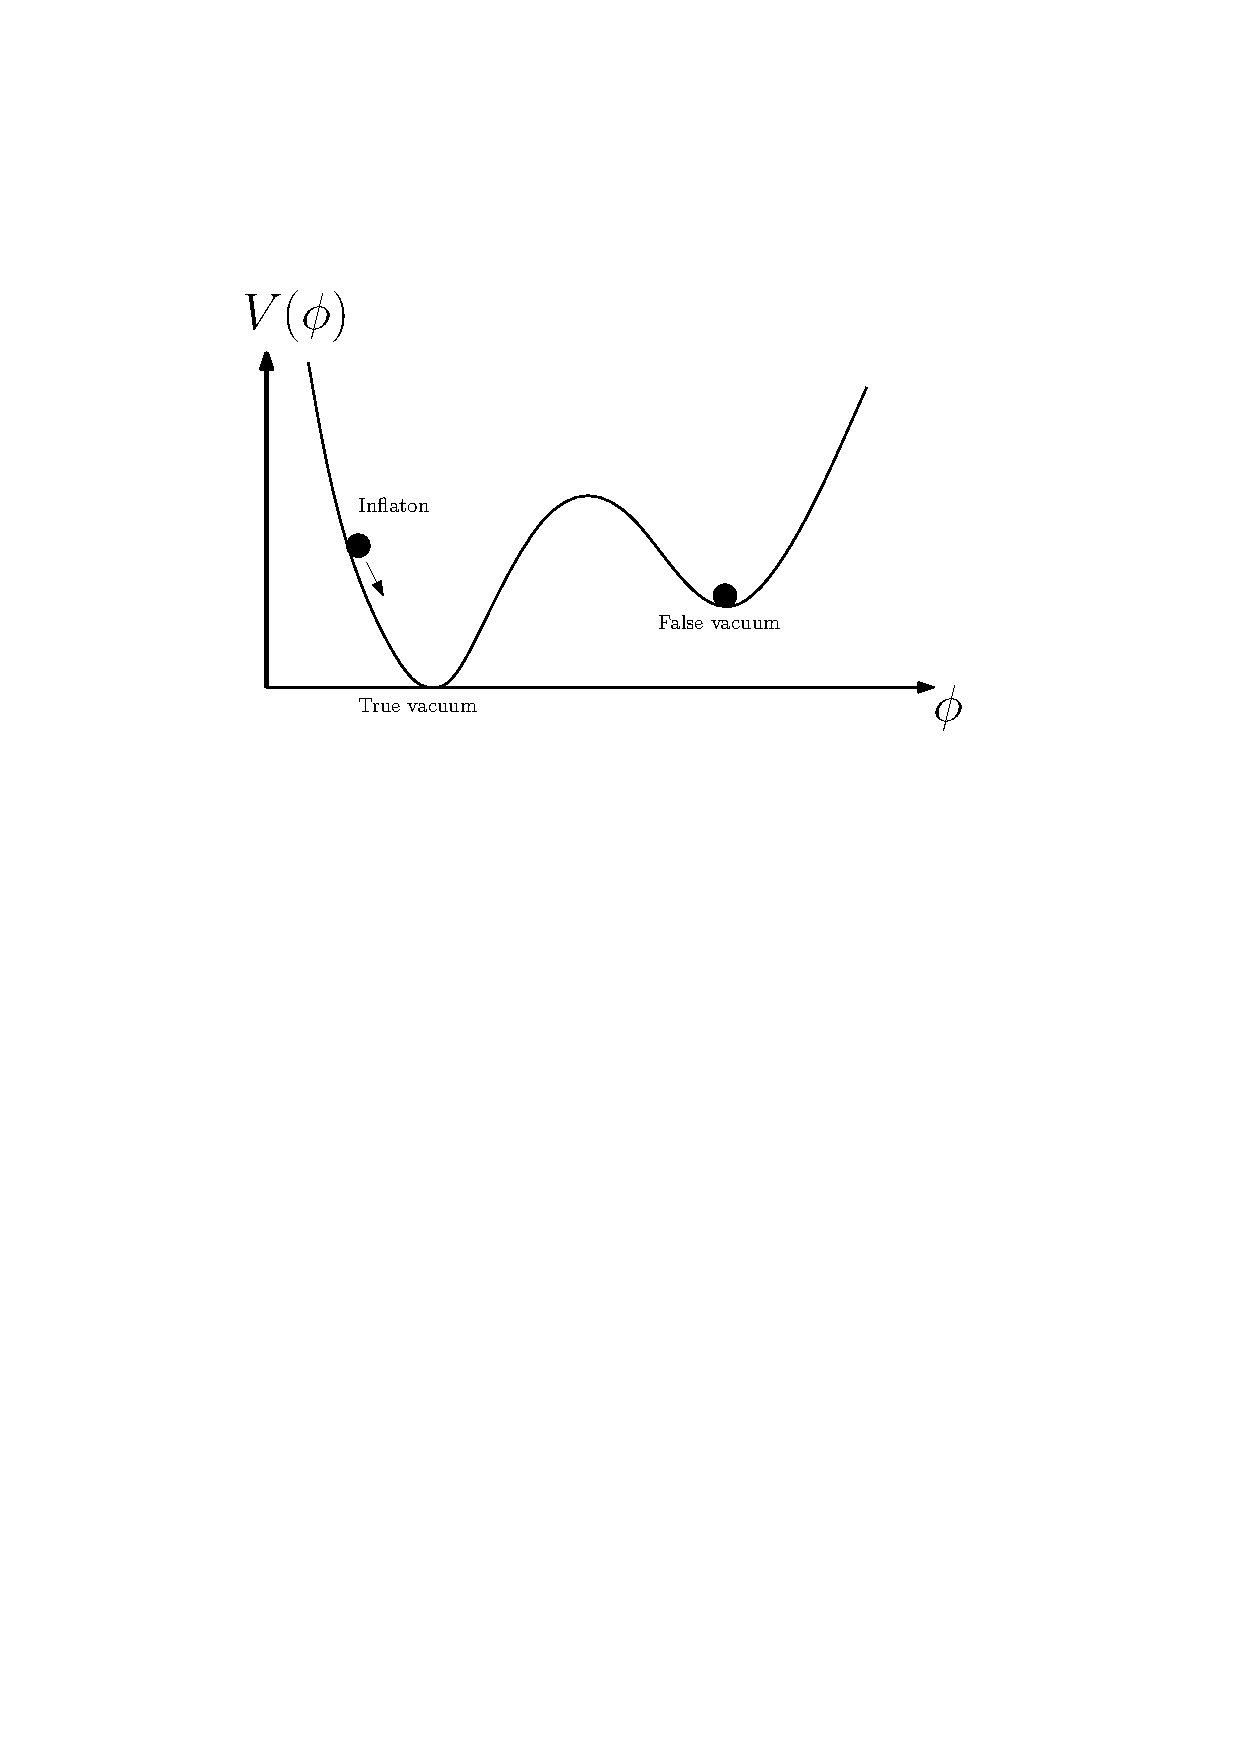
\includegraphics[width=\textwidth]{potential}
  \caption{An example inflationary potential.}
  \label{fig:cos:potential}
\end{figure}

In fact, one does not need a false vacuum, one merely needs the inflaton to be rolling slowly down the potential with its speed small in comparison to the potential energy:
\begin{equation}
  \dot{\phi}^2 \ll V(\phi)
  \label{eqn:cos:slow_roll}
\end{equation}
In this case, one still has the Hubble parameter $H\approx H_0$ being approximately constant and therefore exponential expansion. Since the frictional term in~\eqref{eqn:cos:KG} robs the particle of energy, one finds that in fact these slowly rolling phases are generic attractors for most inflationary potentials. All one requires is that the inflaton begins a reasonable way from the potential minimum.

Thus, a very general scalar particle is capable of triggering a generic exponential accelerated expansion. This epoch of the universe is termed inflation.

\subsection{Reheating}
Inflation finishes when the inflaton reaches its true vacuum, and oscillates about its minimum. One then imagines that the inflaton then decays into more traditional matter in a period called reheating. This is theoretically interesting, and an area of active research, but for the purposes of setting initial conditions on the remainder of the contents of the universe it can often be ignored.




\section{The perturbed universe}
The real universe is not smooth, despite how much of a good approximation that might be. Using the FRW metric as a 0\textsuperscript{th} order approximation, we may expand about these smooth solutions. In general then, we write each quantity as:
\begin{equation}
  X(t,\vx) = X(t) + \delta X(t,\vx)
  \label{eqn:cos:expansion}
\end{equation}
Since in the early universe the perturbations were small $\delta X \ll X$, we may expand all equations to linear order to very high accuracy.

\begin{table}
  \centering
\begin{tabular}{lll}
 \toprule
  Symbol & Definition \\
 \midrule
 \midrule
 $\Phi$ & lapse \\
 $B_i$ & shift \\
 $\Psi$ & (spatial) curvature perturbation  \\
 $E_{ij}$ & (spatial) shear (3-tensor) \\
 \bottomrule
\end{tabular}
\caption{Definitions of terms in the perturbed FRW metric}\label{tab:cos:perturbed_metric}
\end{table}


\subsection{Metric perturbation}
A general perturbation of the FRW metric will take the form:
\begin{equation}
  ds^2 = (1+2\Phi)dt^2 -2a B_i dx^i dt  -a^2 \left[ \left( 1 - 2 \Psi \right)\delta_{ij} + 2E_{ij} \right] dx^i dx^j,
  \label{eqn:cos:FRW_perturb}
\end{equation}
where the various terms in the above expression are defined in Table~\ref{tab:cos:perturbed_metric}, and ${\Phi,B_i,\Psi,E_{ij}\ll1}$ are small. 

\subsection{Matter perturbation}
Perturbations of the matter content will take the form:
\begin{equation}
  \rho = \rho + \delta \rho, \qquad 
  P = P + \delta P, \qquad
  u^\mu = \left[ 1-\Phi, a^{-2} \delta q^i/(\rho+P)\right].
  \label{eqn:cos:matter_perturb}
\end{equation}
The density and pressure perturbations are self-explanatory. The perturbation to the fluid velocity is first chosen so that $u^\mu u_\mu=1$ to first order, and $\delta q^i$ is the perturbation to the momentum density. The advantage of this is that for non-interacting fluids, \delta $\rho$, $\delta P$ and $\delta q^i$ are all additive, as in equation~\eqref{eqn:cos:multi_component}. We have neglected a perturbation to the anisotropic stress. Anisotropic stress may be included if desired, but is typically not a physical phenomenon. 

At some point one must also assume an equation of state for the fluid which provides equations to constrain $P$ and $\rho$. We shall limit ourselves to adiabatic matter, which satisfies:
\begin{equation}
  \frac{\delta P}{\dot{P}} = \frac{\delta\rho}{\dot{\rho}}.
  \label{eqn:cos:adiabatic}
\end{equation}
This is not particularly restrictive, and is naturally satisfied by the equations of state~\eqref{eqn:cos:multi_component}.

The scalar field perturbation is similarly simple:
\begin{equation}
  \phi = \phi + \delta\phi.
\end{equation}

\subsection{Fourier modes and SVT decomposition}
In general, the Einstein equations~\eqref{eqn:cos:einstein_tensor} are non-linear, second order, partial differential equations and are therefore extremely challenging to solve. Perturbing about a background as in the previous section yields linearised versions of the Einstein~\eqref{eqn:cos:einsteins_equations} and conservation equations~\eqref{eqn:cos:SET_conservation}:
\begin{align}
  \delta G_{\mu\nu} &= \frac{1}{\m^2}\delta T_{\mu\nu}
  \label{eqn:cos:einsteins_equations_perturb} \\
  \nabla_\mu\delta T^{\mu}_{\nu} &=0
  \label{eqn:cos:SET_conservation_perturb}
\end{align}
which simplifies matters.  
We may go further and exploit the symmetry of the background unperturbed universe to make life even easier:
\begin{itemize}
  \item Translational invariance of the unperturbed universe means that the Fourier modes of the perturbations do not interact, simply turning spatial derivatives into multiples of wavevectors. 
  \item Further the rotational invariance of  the unperturbed universe means that when the 3-vector and 3-tensor perturbations are decomposed into helicity modes, these helicity modes are also non-interacting.
\end{itemize}
Formally, a general field $\varphi(t,\vx)$ can be written in Fourier modes as:
\begin{align}
  \varphi(t,\vk) &= \int d^3\vx\: \varphi(t,\vx) e^{-i\vk \cdot \vx},\\
  \varphi(t,\vx) &= \int \frac{d^3\vk}{{(2\pi)}^3}\: \varphi(t,\vx) e^{i\vk \cdot \vx}.
\end{align}
A vector field $V_i$ and a symmetric, traceless tensor field $T_{ij}$ can be decomposed into helicity modes as:
\begin{align}
  V_i =& \partial_i V + V_i,   \nonumber\\
  &(\partial^k V_k=0) \\
  T_{ij} =& (\partial_i\partial_j - \frac{\delta_{ij}}{3}\partial^k\partial_k)T + \frac{1}{2}(\partial_i T_j + \partial_j T_i) + T_{ij} \nonumber\\ 
  &(\partial^k T_{ki} = \partial^k T_k = 0),
\end{align}
where $V$ and $T$ are helicity scalars, $V_i$ and $T_i$ are divergenceless 3-vectors and $T_{ij}$ is a divergenceless, symmetric, traceless 3-tensor\footnote{Note the overloaded notation: $V_i$ and $T_{ij}$ mean different things on either side of each equation.}.

We may therefore decompose the vectors $B_i$ and $\delta q_i$ into scalar and vector parts, and the tensor $E_{ij}$ into scalar vector and tensor parts, decoupling the helicity modes into three parallel analyses.

\subsection{Gauge choice}
Observant readers will have noted that there are too many perturbation variables and not enough constraints.
This lack of constraint arises from the fact that the split into background and perturbation $X=X+\delta X$ implied by~\eqref{eqn:cos:expansion} is more subtle than first appears. 

In addition to perturbing the dynamical variables, one can also perturb the coordinate system:
\begin{align}
  t &\rightarrow t + \delta t  
  \label{eqn:cos:gauge_t}
  \\
  x^i &\rightarrow x^i  + \delta x^i ,
  \label{eqn:cos:gauge_x}
\end{align}
where in general the small perturbations $\delta t$ and $\delta x^i$ are functions of time and space.
For a generic scalar field $\varphi = \varphi(t,x^i)$, this coordinate perturbation will cause an alteration of the field value:
\begin{equation}
  \varphi \rightarrow \varphi - \dot{\varphi}\delta t - \partial_i\varphi\delta x^i.
\end{equation}
This means that it is easy to conflate ``true'' perturbations in the variables with coordinate perturbations. In the extreme limit of no dynamical perturbation, one can see that the coordinate transformation~\eqref{eqn:cos:gauge_t}~\&~\eqref{eqn:cos:gauge_t} will in in generate a ``false'' perturbation in $\varphi$ of $\delta\varphi = -\dot{\varphi}\delta t - \partial_i\varphi\delta x^i$.

Careful calculation will show that in fact the transformation of the dynamical variables under~\eqref{eqn:cos:gauge_t}~\&~\eqref{eqn:cos:gauge_t} is in fact:
\begin{align}
  \Phi &\rightarrow \Phi - \delta \dot{t} &
  \Psi &\rightarrow \Psi +H \delta t  \nonumber\\
  B &\rightarrow B + \delta t/a - a\delta \dot{x} &
  B_i &\rightarrow  B_i - a \delta\dot{x}_i  \nonumber\\
  E &\rightarrow E - \delta x &
  E_i & \rightarrow E_i - \delta x_i \nonumber \\
  \delta\rho &\rightarrow \delta\rho - \dot{\rho}\delta t &
  \delta P &\rightarrow \delta P - \dot{P}\delta t \nonumber\\
  \delta q &\rightarrow \delta q - (\rho+P)\delta \dot{x}&
  \delta q^i &\rightarrow \delta q^i - (\rho+P)\delta \dot{x}^i \\
  \delta \phi &\rightarrow \delta \phi - \dot{\phi}\delta t &&\nonumber
\end{align}
By choosing an appropriate coordinate transformation, one can remove the additional dynamical variables that are unconstrained by the Einstein equations. This is typically done by setting some of the perturbation variables equal to zero. This procedure is termed a {\em gauge choice}.\footnote{$\delta X$ is defined as the difference between the value $X$ has in the physical (perturbed) spacetime, and the value $X$ has in the background (unperturbed) spacetime. This can only be done if there is a prescription for identifying points between the two spacetimes, and in the language of differential geometry, this is termed a {\em gauge choice}.}
Examples of popular gauge choices can be found in Table~\ref{tab:cos:gauge_choice}.

Whilst choosing a gauge will give one a set of soluble equations, the question still remains as to whether the perturbations really are ``true'', or in some-way coordinate-dependent. A more robust approach is to avoid the issue entirely and define the gauge independent variables:
\begin{align}
  \Phi^{(B)} &=  \Phi - \dot{T} &
  \Psi^{(B)} &=  \Psi + HT \nonumber \\
  B_i^{(B)} &= B_i - a\dot{E}_i & & \nonumber\\
  \delta\rho^{(B)} &= \delta\rho - \dot{\rho}T &
  \delta P^{(B)} &= \delta P - \dot{P}T & \nonumber\\
  \delta q^{(B)} &= \delta q - (\rho + P)\dot{E} &
  \delta q_i^{(B)} &= \delta q_i - (\rho + P)\dot{E}_i \nonumber \\
  \delta \phi^{(B)} &= \delta \phi - \dot{\phi}T & &
\end{align}
where $T = a^2[\dot{E}-B/a]$. These variables remain unchanged under gauge transformations, and are independent of coordinate perturbations. Any perturbation in these variables cannot be ``gauged away''. Of course, these are not unique as any linear combination of them is also gauge invariant, but the above set results in a reasonable basis. 

Procedurally, one of  the most powerful approaches is to choose the Newtonian gauge ${B=E=E_i=0}$. In this gauge, $X^{(B)}=X^{(\text{Newt.})}$. At the end of the computation, we may note that any equations in $X^{(\text{Newt.})}$ will be manifestly gauge invariant, so we may re-promote all variables $X^{(\text{Newt.})}$ to the gauge-invariant ones $X^{(B)}$.


\begin{table}
  \centering
\begin{tabular}{ll}
 \toprule
  Name & Definition \\
 \midrule
 \midrule
 Synchronous & $\Phi=B=0$ \\
 Newtonian & $B=E=0$ \\
 Uniform density & $\delta\rho=0$ and e.g.\ $E=0$ \\
 Comoving & $\delta q = E = 0$ \\
 Spatially-flat & $\Psi=E=0$ \\
 \bottomrule
\end{tabular}
\caption{Popular gauge choices for the scalar components of the metric}\label{tab:cos:gauge_choice}
\end{table}

\section{Comoving curvature perturbation}

\subsection{Classical behaviour}
It is convenient to examine the gauge invariant variable:
\begin{equation}
  \mathcal{R} = \Psi - \frac{H}{\rho+P}\delta q.
  \label{eqn:cos:CCP}
\end{equation}
This is termed the {\em comoving curvature perturbation}, since in the comoving gauge ($\delta q=0$) $\mathcal{R}=\Psi$.
After some effort, the Einstein equations~\eqref{eqn:cos:einsteins_equations}~\&~\eqref{eqn:cos:einsteins_equations_perturb} and conservation equations~\eqref{eqn:cos:SET_conservation}~\&~\eqref{eqn:cos:SET_conservation_perturb} evaluated using the perturbed metric~\eqref{eqn:cos:FRW_perturb} and the perturbed stress energy tensor~\eqref{eqn:cos:SET_perfect_fluid}~\&~\eqref{eqn:cos:matter_perturb} yields:
\begin{equation}
  \frac{d \log \mathcal{R}}{d \log a} = 
  -\frac{k^2}{a^2(5\rho + 3P)}\frac{\dot{P}}{\dot{\rho}}.
\end{equation}
Given that $\rho,P\sim H^2$, the above equation says that: $\frac{d\log \mathcal{R}}{d\log a} \sim \frac{k^2}{a^2H^2}$. As the universe inflates, $k\ll aH$, and $\mathcal{R}$ ``freezes out'' and becomes constant.

\subsection{Quantum behaviour}
Using the Lagrangians are defined by equations~\eqref{eqn:cos:L_grav}~\&~\eqref{eqn:cos:scalar_field_lagrangian}, we may define the action:
\begin{equation}
  S = \int d^4x\sqrt{|g|}\mathcal{L}_G + \mathcal{L}_\phi.
\end{equation}
If we expand this action to second order in $\mathcal{R}$, we find (after some effort):
\begin{equation}
  S^{(2)} = \int d^4x\: a^3 \frac{\dot{\phi}^2}{H^2}\left[ \mathcal{\dot{R}}^2 -a^{-2}{\left( \delta_i\mathcal{R} \right)}^2 \right]
\end{equation}
Switching to conformal time and defining:
\begin{equation}
  v = z \mathcal{R}, \qquad
  z = \frac{a \dot{\phi}}{H},
\end{equation}
the action becomes:
\begin{equation}
  S^{(2)} = \int d^4x\: \left[ {\left( v^{\prime} \right)}^2 - {\left( \partial_i v \right)}^2 + \frac{z^{\prime\prime}}{z}v^2\right],
\end{equation}
where primes denote derivatives with respect to conformal time.

To quantise, we promote the field variable $v$ to a quantum operator, and write it as a Fourier superposition:
\begin{equation}
  v = \int \frac{d^3k}{{\left( 2\pi \right)}^3}
  \left[ 
    \chi_k^{\phantom\ast}(\eta) a_\vk^{\phantom\dagger}e^{i\vk\cdot\vx} + 
    \chi_k^\ast(\eta) a_\vk^{\dagger}e^{-i\vk\cdot\vx}  
  \right]
\end{equation}
of mode functions $v_\vk = \chi_k a_\vk$
Requiring that the canonical commutator relation:
\begin{equation}
  \left[ a_{\vk^{\phantom\prime}}^{\dagger}, a_{\vk^{\prime}}^{\phantom\dagger}\right] = {\left( 2\pi \right)}^3\delta^{(3)}\left( \vk^{\phantom\prime}-\vk^{\prime} \right),
\end{equation}
holds true, then the wavefunction $\chi_k(\eta)$ must satisfy:
\begin{align}
  \chi_k^{\prime\prime} + \left( k^2 - \frac{z^{\prime\prime}}{z} \right) \chi_k &=0 \\
  {\chi_k^{\phantom\ast}}^{\prime} 
  {\chi_k^{\ast}}^{\phantom\prime} 
  -
  {\chi_k^{\ast}}^{\prime} 
  {\chi_k^{\phantom\ast}}^{\phantom\prime} 
  &= -i.
\end{align}





\section{Statistics of the CMB}
We write a general perturbation to the temperature field of the universe as:
\begin{equation}
  T(t,\vx,\vp) = T(t)\left[ 1+\Theta(t,\vx,\vp) \right]
\end{equation}
Note that the temperature field is anisotropic (i.e.\ has a $\vp$ dependency) on account of the relativistic nature of photons. We may separate this angular dependence by expanding $\Theta$ in spherical harmonics:
\begin{align}
  \Theta(t,\vx,\vp) &= \sum_{\ell=1}^{\infty}\sum_{m=-\ell}^{\ell}a_{\ell m}(t,\vx) Y_{\ell m}(\vp)\\
  a_{\ell m}(t,\vx) &= \int d\Omega Y_{\ell m}(\vp) \Theta(t,\vx,\vp)
  \label{eqn:cos:alm_integral}
\end{align}
We only observe the temperature field here (at $\vx_0$) and now (at $t_0$). By taking sufficiently many measurements in different directions of $\vp$ of the temperature field $\Theta$ we can compute the integral~\eqref{eqn:cos:alm_integral}, to obtain $a_{\ell m}(t_0,\vx_0)$ up to some $\ell_{\max{}}$.\footnote{As a rough guide, if one has $N_\mathrm{pix}$ independent pixels, there are ${(\ell_{\max{}}+1)}^2$ different $a_{\ell m}$'s to measure, so $\ell_{\max{}} \sim \sqrt{N_\mathrm{pix}}$.}

In general, theories do no predict specific values of $a_{\ell m}$, but merely tell us about the statistical distribution on which they are drawn. At each value of $\ell$, the $(2\ell + 1)$ observations $\{a_{\ell m}:m=-\ell\cdots\ell\}$ are typically independent realisations of the same random variable. Their mean value is zero, but they will have some non-zero variance:
\begin{equation}
  \left\langle a_{\ell m} \right\rangle = 0, \qquad
  \left\langle a_{\ell m} a_{\ell^\prime m^\prime}\right\rangle = \delta_{\ell \ell^\prime} \delta_{m m^\prime} C_\ell
\end{equation}
Note then that the error therefore in the sample variance obeys:
\begin{equation}
  \left( \frac{\Delta C_\ell}{C_\ell} \right) = \sqrt{\frac{2}{2\ell+1}}.
\end{equation}
This means that on larger angular scales, we have fewer $a_{\ell m}$'s to use to compute the sample variance, and hence have a larger sample error. This is a manifestation of {\em cosmic variance}, resulting from the fact that we only have one universe to observe. 

Computing the theoretical predictions of these $C_\ell$'s from a given cosmology is complicated, requiring one to evolve the contents of the universe from some initial early time through the hot big bang era, past the surface of last scattering at recombination and all the way to the sky we see today. Treating this calculation fully is beyond the scope of this thesis, but it suffices to say that this is now extremely well understood physics, and a full set of $C_\ell$'s can be computed for a given cosmology using codes such as \CAMB{} in a matter of seconds.

\clearpage{}

